The inverse discrete-time Fourier transform can be used for filter
design purposes. It is possible to specify a filter in frequency
domain $\mathcal{H}(\hat{\omega})$, and then use an inverse Fourier
transform to obtain the impulse response $h[n]$ of the filter with
these properties. However, this often leads to filters that are
infinitely long and therefore impossible to realize. In practice, the
issue of infinitely long filters can be overcome by truncating
the impulse response into one that has a finite length.

This chapter will only discuss ideal and tapered windows in the
context of discrete-time signals. We will first go through several
important ideal filters and derive their impulse responses. We will
then discuss various strategies for truncating and tapering these
into finite length filters.

\section{Ideal filters}

It is possible to specify a filter in frequency domain. In many cases,
one knows what sort of frequency response is needed. The basic recipe
is to inverse DTFT the desired frequency response to obtain a time
domain impulse response. In this section, we'll go through some basic
ideal filters.

\subsection{Example: Ideal low-pass filter}

An ideal low-pass filter has the following spectral response:
\begin{equation}
  \mathcal{H}_{\mathrm{LP}}(\hat{\omega}) = \left\{ \begin{array}{cc}
    1 & |\hat{\omega}| < \hat{\omega}_0           \\
    0 & \hat{\omega_0} \le |\hat{\omega}| \le \pi
  \end{array}\right.\,\,.
\end{equation}
\begin{marginfigure}
  \begin{center}
    \begin{tikzpicture}
      \begin{axis}[width=7cm,height=6cm,ymin=0,xmin=-2.5,ymax=1.2,xmax=2.5,  yticklabels={,,},
          xtick={-2,-1,1,2},
          xticklabels={$-\pi$,$-\omega_0$,$\omega_0$,$\pi$},
          ylabel={$\He$},
          xlabel=$\hat{\omega}$, axis lines = center]

        \addplot[mark=none,color=blue] coordinates {
            (-2,0)
            (-1,0)
            (-1,1)
            (1,1)
            (1,0)
            (2,0)
          };

        %\draw [gray, thick] (axis cs:-1,0.0) rectangle (axis cs:1,1.4);
        %   \node at (axis cs:-0.4,1.1) [above, font={\footnotesize}]{$\mathcal{H}_{\mathrm{LP}}(e^{i\hat{\omega}})$};
      \end{axis}
    \end{tikzpicture}
  \end{center}
  \caption{The frequency response of an ideal low pass filter, which filters out signals with normalized frequencies larger than $|\hat{\omega}|>\hat{\omega}_0$}
\end{marginfigure}
In order to determine the filter coefficients, one needs to inverse DTFT the frequency response:
\begin{align}
  h[n] & =\frac{1}{2\pi}\int_{-\pi}^{\pi}\mathcal{H}_{\mathrm{LP}}(\hat{\omega}) e^{i\hat{\omega}n} d\hat{\omega} \\
       & = \frac{1}{2\pi}\int_{-\hat{\omega}_0}^{\hat{\omega}_0} e^{i\hat{\omega}n}d\hat{\omega}                  \\
       & = \frac{1}{2\pi} \left.\frac{e^{i\hat{\omega}n}}{i n}\right\vert_{-\hat{\omega}_0}^{\hat{\omega}_0}      \\
       & =\frac{1}{\pi n}\frac{1}{2i}(e^{i\hat{\omega}_0 n} - e^{-i\hat{\omega}_0n})                              \\
       & = \frac{\sin(\hat{\omega}_0 n)}{\pi n}\,\,.
\end{align}
The impulse response for this ideal filter is infinitely long, but it
is damped by a factor of $1/n$. There is also an indeterminate value
at $n=0$, which can be determined using L'H\^opital's rule.
\begin{marginfigure}
  \begin{center}
    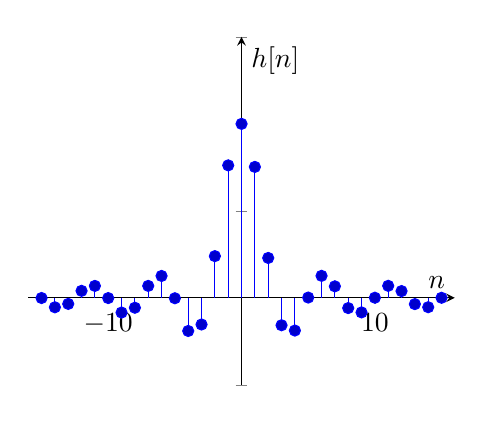
\begin{tikzpicture}
      \begin{axis}[domain=-15:15,
          width=7cm,
          ymin=-0.2,
          ymax=0.6,
          height=6cm,
          xmax=16,
          xmin=-16,
          %                       xtick={-2,2},
          %                      xticklabels={$-n_0$,$n_0$},
          yticklabels={,,},
          xlabel=$n$,
          ylabel={$h[n]$},
          axis lines = center]
        \addplot+[ycomb,samples=31]{sin(0.4*3.14*deg(x+0.01))/(3.14*(x+0.01)) };
      \end{axis}
    \end{tikzpicture}
  \end{center}
  \caption{The impulse response of an ideal low-pass filter.}
  \label{fig:ideal_lp_ir}
\end{marginfigure}
\begin{align}
  \lim_{x\rightarrow c} \frac{f(x)}{g(x)}                   & = \lim_{x\rightarrow c} \frac{f'(x)}{g'(x)}                             \\
  \lim_{n\rightarrow 0} \frac{\sin(\hat{\omega}_0n)}{\pi n} & = \lim_{n\rightarrow 0} \frac{\hat{\omega}_0\cos(\hat{\omega}_0n)}{\pi} \\
                                                            & = \frac{\hat{\omega}_0}{\pi} \,\,.
\end{align}
Therefore, the ideal low-pass filter is defined as:
\begin{equation}
  \boxed{
    h[n]=\frac{\sin(\hat{\omega}_0 n)}{\pi n}  \xleftrightarrow{\mathcal{F}} \He = u(\hat{\omega}+\hat{\omega}_0)-u(\hat{\omega}-\hat{\omega}_0)\,\,.
  }
\end{equation}
The impulse response for an ideal low-pass filter with $\hat{\omega}_0
  = 0.4\pi$ is shown in Figure \ref{fig:ideal_lp_ir}.

The function $\sin(\pi x)/\pi x$ is often referenced to as the $\mathrm{sinc}$-function:
\begin{equation}
  \mathrm{sinc}(\theta) = \frac{\sin(\pi\theta)}{\pi \theta}\,\,.
\end{equation}
Sometimes it is useful to express the ideal low-pass using a sinc
function, as numerical implementations of this function take into
account the limiting behavior at $\hat{\omega}=0$ automatically.


\subsection{Example: Ideal high-pass filter}

An ideal high-pass filter with a cutoff at $\hat{\omega}_0$ is defined as:
\begin{equation}
  \mathcal{H}_{\mathrm{HP}}(\hat{\omega}) = \left\{ \begin{array}{cc}
    0 & |\hat{\omega}| < \hat{\omega}_0     \\
    1 & \omega_0 \le |\hat{\omega}| \le \pi
  \end{array}\right.\,\,.
\end{equation}
\begin{marginfigure}
  \begin{center}
    \begin{tikzpicture}
      \begin{axis}[width=7cm,height=6cm,ymin=0,xmin=-2.5,ymax=1.5,xmax=2.5,  yticklabels={,,},
          xtick={-2,-1,1,2},
          xticklabels={$-\pi$,$-\omega_0$,$\omega_0$,$\pi$},
          ylabel=$\He$,
          xlabel=$\hat{\omega}$, axis lines = center]

        %\draw [gray, thick] (axis cs:-1,0.0) rectangle (axis cs:1,1.4);

        \addplot[mark=none,color=blue] coordinates {
            (-2,1)
            (-1,1)
            (-1,0)
            (1,0)
            (1,1)
            (2,1)
          };
        %   \node at (axis cs:-0.4,1.1) [above, font={\footnotesize}]{$\mathcal{H}_{\mathrm{HP}}(e^{i\hat{\omega}})$};
      \end{axis}
    \end{tikzpicture}
  \end{center}
  \caption{The frequency response of an ideal high-pass filter.}
\end{marginfigure}
To obtain the time domain impulse response $h[n]$, we perform an
inverse DTFT, much in the same way as we did for the ideal low pass
filter:
\begin{align}
  h[n] & = \frac{1}{2\pi}\int_{-\pi}^{\pi} \mathcal{H}_{\mathrm{HP}}(\hat{\omega}) e^{i\hat{\omega}n} d\hat{\omega}                                     \\
       & =\frac{1}{2\pi}\left[\int_{-\pi}^{-\omega_0} e^{i\hat{\omega}n} d\hat{\omega} + \int_{\omega_0}^{\pi} e^{i\hat{\omega}n} d\hat{\omega} \right] \\
       & =\frac{1}{2\pi ni}\left[ e^{-i\hat{\omega}_0 n} - e^{-i\pi n} + e^{i\pi n} - e^{i\hat{\omega}_0 n} \right]                                     \\
       & =\frac{1}{\pi n}\left[\sin(\pi n) - \sin(\hat{\omega}_0  n) \right]\,\,.
\end{align}
Here we need to be careful when $n=0$. While $\sin(\pi n)/\pi n = 0$ when $n\ne 0$, when $n=0$, using L'H\^opital's rule, we get:
\begin{equation}
  \lim_{n\rightarrow 0} \frac{\sin(\pi n)}{\pi n} = 1\,\,.
\end{equation}
Therefore, the impulse response of the ideal high-pass filter is:
\begin{equation}
  \boxed{
  h[n]=\delta[n] - \frac{\sin(\hat{\omega}_0 n)}{\pi n} \xleftrightarrow{\mathcal{F}} \He = 1-[u(\hat{\omega}+\omega_0)-u(\hat{\omega}-\omega_0)]
  }
\end{equation}
which is another way of saying all but the ideally low pass filtered
signal.

\begin{marginfigure}
  \begin{center}
    \begin{tikzpicture}
      \begin{axis}[width=7cm,height=6cm,ymin=0,xmin=-2.5,ymax=1.5,xmax=2.5,  yticklabels={,,},
          xtick={-2,-1.5,-0.5,0.5,1.5,2},
          xticklabels={$-\pi$,$-\omega_1$,$-\omega_0$,$\omega_0$,$\omega_1$,$\pi$},
          ylabel=$\He$,
          xlabel=$\hat{\omega}$, axis lines = center]

        \addplot[mark=none,color=blue] coordinates {
            (-2,0)
            (-1.5,0)
            (-1.5,1)
            (-0.5,1)
            (-0.5,0)
            (0.5,0)
            (0.5,1)
            (1.5,1)
            (1.5,0)
            (2,0)
          };
        %   \node at (axis cs:-0.4,1.1) [above, font={\footnotesize}]{$\mathcal{H}_{\mathrm{BP}}(e^{i\hat{\omega}})$};
      \end{axis}
    \end{tikzpicture}
  \end{center}
  \caption{The frequency response of an ideal band-pass filter.}
  \label{fig:ideal_bp_fr}
\end{marginfigure}

\subsection{Example: Ideal band-pass filter}
An ideal band-pass filter has a non-zero frequency response only on a
narrow frequency range (passband). For a real-valued passband
filter, one needs to include the positive and negative frequency passbands.
The specification for an ideal band-pass filter that
only lets through real-valued signals with frequencies between $\omega_0$ and
$\omega_1$ is:
\begin{equation}
  \mathcal{H}_{\mathrm{BP}}(\hat{\omega}) = \left\{ \begin{array}{cc}
    1 & \hat{\omega}_0 < |\hat{\omega}| < \hat{\omega}_1 \\
    0 & \mathrm{otherwise}
  \end{array}\right.\,\,.
\end{equation}
The frequency response is shown in Figure \ref{fig:ideal_bp_fr}.

This has the impulse response given by:
\begin{align}
  h[n] & = \frac{1}{2\pi}\int_{-\pi}^{\pi} \mathcal{H}_{\mathrm{BP}}(\hat{\omega}) e^{i\hat{\omega}n} d\hat{\omega}                                                                       \\
       & =\frac{1}{2\pi}\left[\int_{-\hat{\omega}_1}^{-\hat{\omega}_0} e^{i\hat{\omega}n} d\hat{\omega} + \int_{\hat{\omega}_0}^{\hat{\omega}_1} e^{i\hat{\omega}n} d\hat{\omega} \right] \\
       & =\frac{1}{2\pi ni}\left[ e^{-i\hat{\omega}_0 n} - e^{-i\omega_1 n} + e^{i\omega_1 n} - e^{i\hat{\omega}_0 n} \right]                                                             \\
       & = \frac{\sin(\hat{\omega}_1 n)}{\pi n}-\frac{\sin(\hat{\omega}_0 n)}{\pi n}\,\,.
\end{align}
Again, using L'H\^opital's rule, we obtain the behavior at $n=0$:
\begin{equation}
  h[0]=(\hat{\omega}_1 - \hat{\omega}_0)/\pi\,\,.
\end{equation}

Similarly, it is possible to determine the impulse response for
an ideal band-stop filter, which has zero response between $\omega_0$
and $\omega_1$, but lets through signals at all other frequencies. We
leave this as an exercise to the reader.

\subsection{Example: Ideal point frequency filter}
\label{pointfreq}

A filter, which is selective to only one frequency $\hat{\omega}_0$:
\begin{equation}
  \boxed{
    h[n]=\frac{1}{2\pi} e^{i\hat{\omega}_0 n} \xleftrightarrow{\mathcal{F}} \He = \delta(\hat{\omega}-\hat{\omega}_0)\,\,.
  }
\end{equation}
Here $\delta(x)$ is the Dirac delta function. The impulse response of
such a filter can be obtained using the IDTFT (for $|\omega_{0}|<\pi$:
\begin{align}
  h[n] & =\frac{1}{2\pi}\int_{-\pi}^{\pi} \delta(\hat{\omega}-\hat{\omega}_0) e^{i\hat{\omega}n} d\hat{\omega} \\
       & = \frac{1}{2\pi} e^{i\hat{\omega}_0 n}\,\,.
\end{align}
This filter is constant in magnitude, i.e., $|h[n]|=(2\pi)^{-1}$, and
infinitely long. The filter is a complex sinusoid, with frequency
matched to the signal frequency $\hat{\omega}_0$.

\subsection{Example: Real-valued point frequency filter}

The real-valued single frequency filter is actually a filter that
lets through two frequencies. The positive and negative frequency
component $\hat{\omega}_0$ and $-\hat{\omega}_0$.
\begin{equation}
  \boxed{
    h[n] = \frac{1}{\pi}\cos(\hat{\omega}_0 n)  \xleftrightarrow{\mathcal{F}}  \He = \delta(\hat{\omega}-\hat{\omega}_0) + \delta(\hat{\omega}+\hat{\omega}_0)\,\,.
  }
\end{equation}
\begin{proof}
  \begin{align}
    h[n] & =\frac{1}{2\pi}\int_{-\pi}^{\pi} \delta(\hat{\omega}-\hat{\omega}_0) e^{i\hat{\omega}n} d\hat{\omega} + \frac{1}{2\pi}\int_{-\pi}^{\pi} \delta(\hat{\omega}+\hat{\omega}_0) e^{i\hat{\omega}n} d\hat{\omega} \\
         & = \frac{1}{2\pi} (e^{i\hat{\omega}_0 n}+e^{-i\hat{\omega}_0 n})                                                                                                                                              \\
         & = \frac{1}{\pi}\cos(\hat{\omega}_0 n)\,\,.
  \end{align}
\end{proof}
The ideal point-frequency impulse response will be later revisited
when dealing with discrete Fourier transforms as filter banks.

\section{Fractional sample delay}
An important elementary filter is the time-shift filter, which has an impulse response
\begin{equation}
  h[n] = \delta[n-n_0]\,\,.
\end{equation}
\begin{marginfigure}
  \begin{center}
    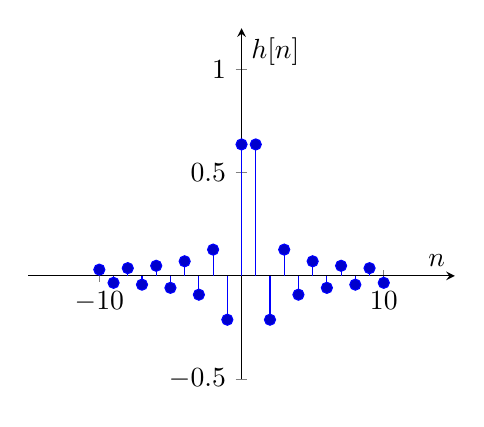
\begin{tikzpicture}
      \begin{axis}[width=7cm,domain=(-10:10), samples=21, xmin=-15,xmax=15, ymin=-0.5,ymax=1.2,
          legend style={draw=none,at={(.99,.1)},anchor=south east},
          xlabel={$n$},
          ylabel={$h[n]$},
          axis x line=center,
          axis y line=middle,
        ]
        \addplot+[ycomb,blue] {sin(deg(3.14*(x-0.5)))/(3.14*(x-0.5))};
      \end{axis}
    \end{tikzpicture}
  \end{center}
  \caption{Fractional sample delay filter impulse response $h[n]$, which delays the signal by half a sample. This filter is infinitely long.}
  \label{fig:frac_samp_delay_ex}
\end{marginfigure}

This filter delays the signal by $n_0$ samples. We already determined earlier that time-delay
is equivalent to a linear phase slope in
frequency domain:
\begin{align}
  \mathcal{H}(\hat{\omega}) & = \sum_{n=-\infty}^{\infty}\delta[n-n_0]e^{-i\hat{\omega}n} \\
                            & =e^{-i\hat{\omega}n_0}\,\,.
\end{align}
We can now use this to derive the impulse response of a fractional sample delay filter,
which delays the signal by a real-valued number of samples $n_0 \in \mathbb{R}$:
\begin{equation}
  \boxed{
    h[n] =\frac{\sin(\pi[n-n_0])}{\pi(n-n_0)} \xleftrightarrow{\mathcal{F}} \He = e^{-i\hat{\omega}n_0}\,\,.
  }
\end{equation}
For the proof, we need to evaluate the inverse DTFT of the frequency domain specification of a time-shift
$\mathcal{H}(\hat{\omega})=e^{-i\hat{\omega}n_0}$:
\begin{align}
  x[n] & = \frac{1}{2\pi}\int_{-\pi}^{\pi} e^{-i\hat{\omega}n_0} e^{i\hat{\omega}n}d\hat{\omega}               \\
       & = \frac{1}{2\pi}\int_{-\pi}^{\pi}  e^{i\hat{\omega}(n-n_0)}d\hat{\omega}                              \\
       & =\left.\frac{1}{2\pi} \frac{e^{i\hat{\omega}(n-n_0)}}{i(n-n_0)}\right \vert_{\hat{\omega}=-\pi}^{\pi} \\
       & = \frac{1}{\pi(n-n_0)}\frac{1}{2i}(e^{i\pi(n-n_0)}-e^{-i\pi(n-n_0)})                                  \\
       & = \frac{\sin(\pi[n-n_0])}{\pi[n-n_0]}\,\,.
\end{align}
Figure \ref{fig:frac_samp_delay_ex} shows the impulse response of a
filter that delays a signal by $n_0=0.5$, that is by half a sample. It
would be difficult to define this filter in time domain, but
relatively straightforward using the frequency domain specification,
which is inverse discrete Fourier transformed into time domain to obtain
an impulse response.

It can be shown that for integer values $n_0 \in \mathbb{Z}$, the
impulse response simplifies to
\begin{equation}
  \frac{\sin(\pi[n-n_0])}{\pi(n-n_0)}=\delta[n-n_0]\,\,,
\end{equation}
but this would be easy to define already in time domain.


\section{Tapered ideal filters}

Ideal filters for discrete-time signals, as discussed in the
discrete-time Fourier transform chapter, are impossible to
realize. This is because ideal filters require an infinitely long
impulse response $h[n]$.

In practical applications, finite length filters have to be used.
One method for designing filters is to take these infinitely
long ideal filters and truncate these to get a filter with finite length.
Approximating an ideal filter with an FIR filter can be accomplished by using \emph{\index{window functions}{window
    functions}} or \emph{\index{tapering windows}{tapering windows}}.
A window function is a function that is 0 outside an interval,
so the effect of multiplying with a window function is that the window
function truncates the filter, making it finite.

If $h[n]$ is an ideal filter centered at $n=0$, a windowed version of
this filter is obtained by multiplying the ideal filter with a window
function $w(n)$ of length $N$:
\begin{equation}
  h_{w}[n] = w(n)h[n-N/2],
  \label{eq:windowed_filter}
\end{equation}
After this, the non-zero amplitude portion of the impulse response
$h_{w}[n]$ is finite length and the filter $h_w[n]$ is a finite impulse
response filter that can be applied in practice to a signal.

\begin{marginfigure}
  \begin{center}
    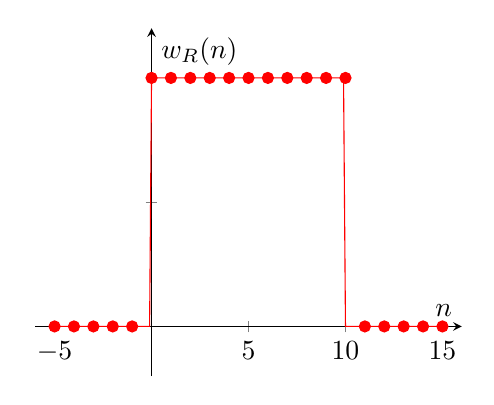
\begin{tikzpicture}
      \begin{axis}[domain=-5:15,samples=21,
          width=7cm,
          ymax=1.2,
          ymin=-0.2,
          height=6cm,
          xmax=16,
          xmin=-6,
          %                       xtick={-2,2},
          %                       xticklabels={$-n_0$,$n_0$},
          yticklabels={,,},
          xlabel=$n$,
          ylabel={$w_R(n)$},
          axis lines = center]
        \addplot+[only marks,red,mark options={red}]{ 1*(x>=0)*(x<=10) };
        \addplot[red,domain=-5:15,samples=201]{ 1*(x>=0)*(x<10) };
      \end{axis}
    \end{tikzpicture}
    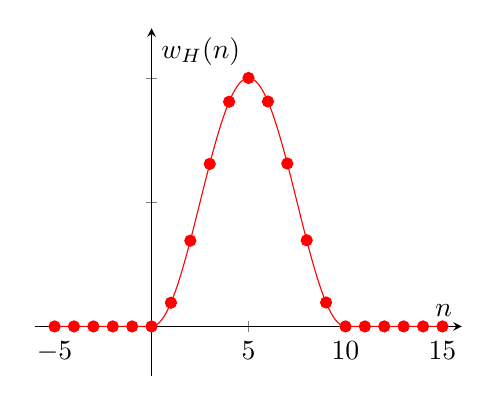
\begin{tikzpicture}
      \begin{axis}[domain=-5:15,samples=21,
          width=7cm,
          ymax=1.2,
          ymin=-0.2,
          height=6cm,
          xmax=16,
          xmin=-6,
          %                       xtick={-2,2},
          %                       xticklabels={$-n_0$,$n_0$},
          yticklabels={,,},
          xlabel=$n$,
          ylabel={$w_H(n)$},
          axis lines = center]
        %\addplot+[ycomb]{ (0.54+0.46*cos(deg(2.0*3.14*(x-4)/9.0)))*(x>=0)*(x<9) };
        \addplot+[only marks,red,mark options={red}]{ sin(deg(3.14*x/10))*sin(deg(3.14*x/10))*(x>=0)*(x<10) };
        \addplot[red,domain=-5:15,samples=201]{ sin(deg(3.14*x/10))*sin(deg(3.14*x/10))*(x>=0)*(x<10) };
      \end{axis}
    \end{tikzpicture}
  \end{center}
  \caption{Top: Rectangular window. Bottom: Hann window. In both cases, the length of the window function is $N=10$.}
  \label{fig:window_functions}
\end{marginfigure}

There are two main effects that you need to be aware of when using
Equation \ref{eq:windowed_filter} to create a truncated finite length
filter. Firstly, there is a time delay of $N/2$ introduced by the
windowing operation. This results in a time shift when applying this
filter. Secondly, due to time-frequency ambiguity, this type of
practical filter will have finite spectral resolution. It is
impossible to achieve a perfectly sharp filter cutoff using a
practical filters.

\section{Rectangular window}

The most basic type of window function is the rectangular window. If
the length of the filter is $N$, the window function evaluates to:
\begin{equation}
  w_{R}[n] =\left\{ \begin{array}{cc}
    1 & 0 \le n \le N-1     \\
    0 & \mathrm{otherwise}.
  \end{array}
  \right.
\end{equation}
This window function just selects $N$ central points of an infinitely
long impulse response $h[n]$.  The top panel of Figure
\ref{fig:window_functions} shows a rectangular window function.


\section{Tapered window}

The window function can also be tapered in such a way that the
amplitude of the window is smoothly reduced to zero near the edges of
the window. This results in better rejection of out of band signals,
at the expense of slightly broadening sharp frequency domain
features.

One example of a good tapered window function is the Hann window. A
Hann window of length $N$ is defined as:
\begin{equation}
  w_{H}[n] =\left\{ \begin{array}{cc}
    \sin^2(\pi n/N) & 0 \le n \le N-1     \\
    0               & \mathrm{otherwise}.
  \end{array}
  \right.
  \label{eq:hann_window_def}
\end{equation}
A Hann window is shown on the bottom panel of Figure
\ref{fig:window_functions}.

A selection of commonly used window function implementations can be
found in the \verb|scipy.signal| module. This includes an
implementation of the Hann window function\sidenote{The Wikipedia page
  on Window functions \url{https://en.wikipedia.org/wiki/Window_function}
  contains a relatively comprehensive visual catalog of the frequency
  responses of different tapering window functions.}.


\section{Example: Frequency selective filter}

\begin{marginfigure}
  \begin{center}
    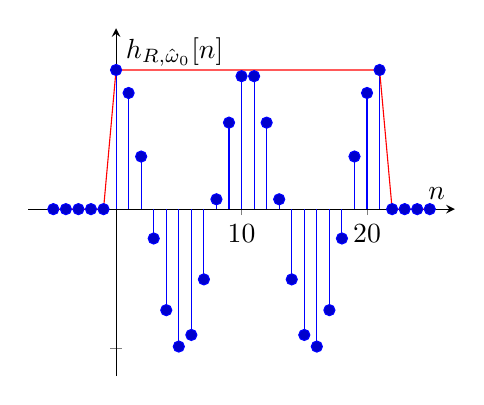
\begin{tikzpicture}
      \begin{axis}[domain=-5:25,samples=31,
          width=7cm,
          ymax=1.3,
          ymin=-1.2,
          height=6cm,
          xmax=27,
          xmin=-7,
          %                       xtick={-2,2},
          %                       xticklabels={$-n_0$,$n_0$},
          yticklabels={,,},
          xlabel=$n$,
          ylabel={$h_{R,\hat{\omega}_0}[n]$},
          axis lines = center]
        \addplot+[ycomb]{ cos(deg(2.0*0.3*(x-21.0/2.0)))*(x>=0)*(x<22) };
        \addplot[red]{ (x>=0)*(x<=21) };
      \end{axis}
    \end{tikzpicture}
    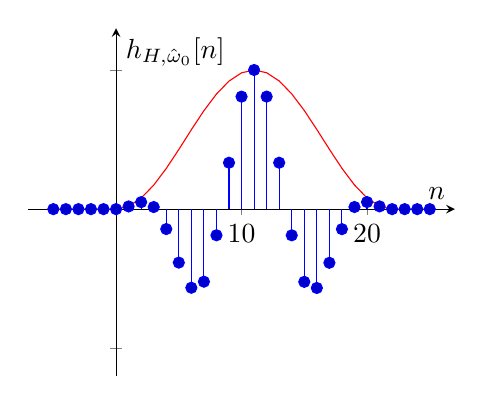
\begin{tikzpicture}
      \begin{axis}[domain=-5:25,samples=31,
          width=7cm,
          ymax=1.3,
          ymin=-1.2,
          height=6cm,
          xmax=27,
          xmin=-7,
          %                       xtick={-2,2},
          %                       xticklabels={$-n_0$,$n_0$},
          yticklabels={,,},
          xlabel=$n$,
          ylabel={$h_{H,\hat{\omega}_0}[n]$},
          axis lines = center]
        \addplot+[ycomb]{ cos(deg(2.0*0.3*(x-22.0/2)))*sin(deg(3.14*x/22))*sin(deg(3.14*x/22))*(x>=0)*(x<22) };
        \addplot[red]{ sin(deg(3.14*x/22))*sin(deg(3.14*x/22))*(x>=0)*(x<22) };
      \end{axis}
    \end{tikzpicture}

  \end{center}
  \caption{Top: Frequency selective filter impulse response using a rectangular window. Bottom: Frequency selective
    filter impulse response using a Hann window. In both cases, the length of the window function is $N=22$.
    The window functions $w(n)$ are shown in red, and the filter impulse response in blue.}
  \label{fig:window_functions2}
\end{marginfigure}


The ideal point-frequency filter for a real-valued signal with frequency
$\hat{\omega}_0$ was shown in the discrete-time Fourier transform
chapter to be:
\begin{equation}
  h[n] = \cos(\hat{\omega}_0 n)
\end{equation}
This is an infinitely long filter, and therefore it is not possible to
implement this filter in practice. The windowed version of this filter
of length $N$ in the case of a rectangular window function would be:
\begin{equation}
  h_{R,\hat{\omega}_0}[n] =\left\{ \begin{array}{cc}
    \cos(\hat{\omega}_0 (n-N/2)). & 0 \le n \le N-1     \\
    0                             & \mathrm{otherwise}.
  \end{array}
  \right.
\end{equation}
and using the Hann window:
\begin{equation}
  h_{H,\hat{\omega}_0}[n] =\left\{ \begin{array}{cc}
    \sin^2(\pi n/N)\cos(\hat{\omega}_0 (n-N/2)) & 0\le n \le N-1      \\
    0                                           & \mathrm{otherwise}.
  \end{array}
  \right.
\end{equation}
The Python code in Listing \ref{lst:frequency_selective} shows an
implementation of a frequency selective filter using a rectangular and
Hann window. The plot produced is shown in Figure
\ref{fig:frequency_selective}.

The key difference between the rectangular windowed and the Hann
windowed filter is the rejection of signals outside the frequencies that
we are trying to filter. A rectangular filter has significantly worse
rejection of out-of-band frequencies compared to the Hann windowed
filter. This is why usually tapered window functions are used.

\begin{figure}
  \begin{center}
    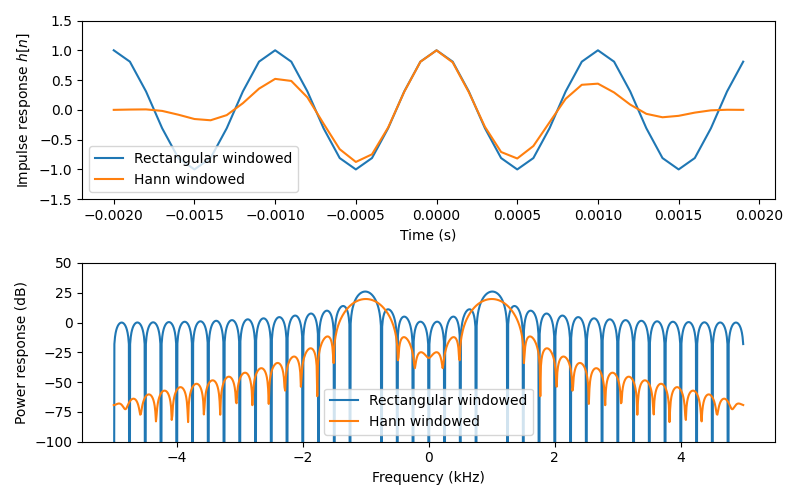
\includegraphics[width=\textwidth]{code/022_window_functions/freq_filter.png}
  \end{center}
  \caption{The impulse response and magnitude response of a frequency selective filter,
    which selects real-valued signals with frequencies $f_0=1$ kHz.
    Top: The impulse response of the rectangular and Hann windowed impulse response.
    Bottom: the power response of the same filters.
    The Hann tapered filter has significantly better rejection of spectral
    components with frequencies outside $f_0=1e3$. However, the rectangular
    windowed filter has a slightly narrower main lobe near the 1 kHz frequency
    that the filter is designed to pass through.
    Due to time-frequency uncertainty, the filter has a finite width.}
  \label{fig:frequency_selective}
\end{figure}


\lstinputlisting[language=Python, caption={\texttt{022\_window\_functions/frequency\_selective.py}}, label=lst:frequency_selective]{code/022_window_functions/frequency_selective.py}

\section{Example: Low-pass filter}

In the discrete-time Fourier transform chapter, we derived the impulse response for an ideal low-pass filter:
\begin{equation}
  h[n] = \frac{\sin(\hat{\omega}_0 n)}{\pi n}.
\end{equation}
This is an infinitely long filter, so the only way to implement this
in practice is to use a windowed version of the ideal impulse
response:
\begin{equation}
  h_w[n] = w(n)\frac{\sin(\hat{\omega}_0 [n-N/2])}{\pi [n-N/2]}.
\end{equation}
The Python code in Listing \ref{lst:windowed_lpf} shows how this is
done in practice. The program evaluates the impulse response of a
Hann windowed ideal low-pass filter and shows the magnitude response
in dB scale. The output of this program is shown in Figure
\ref{fig:lpf_hann}. While this filter does not perfectly remove
spectral components with frequencies outside the passband, it does a
pretty decent job. For example, frequencies $\hat{\omega}=\pm \pi$ are
reduced in power by a factor larger than $10^{12}$.

\begin{figure}
  \begin{center}
    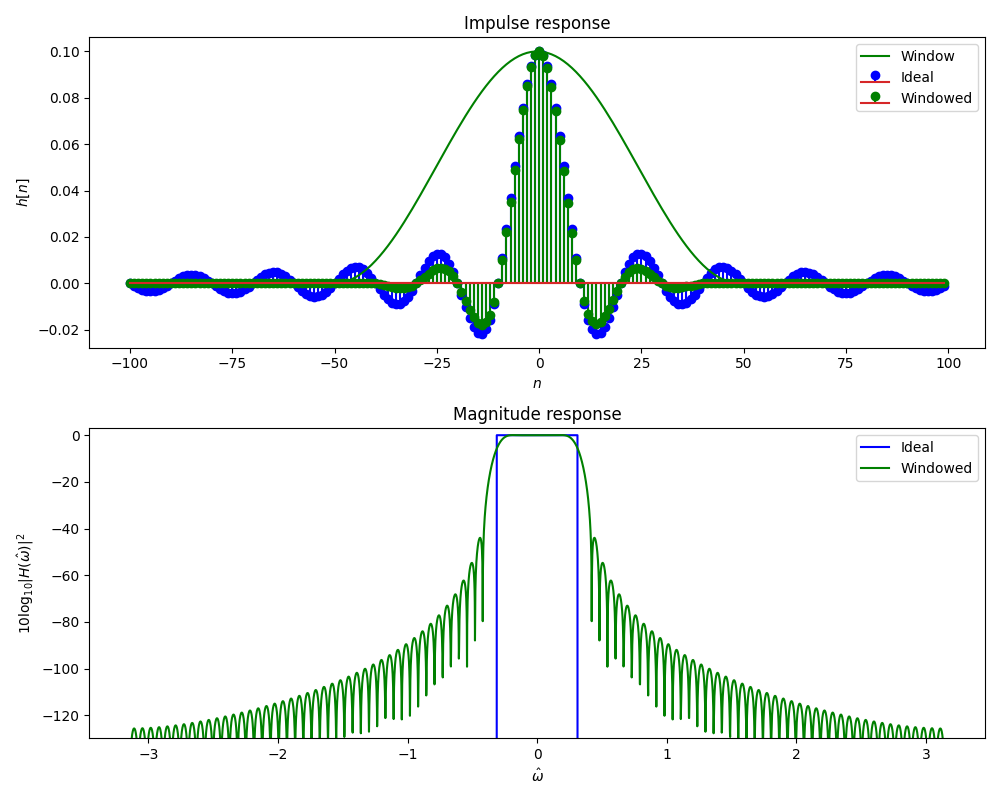
\includegraphics[width=\textwidth]{code/022_window_functions/windowed_lpf.png}
  \end{center}
  \caption{The impulse response and power response of a windowed
    low-pass filter. Top: the impulse response of the ideal filter is
    shown in blue, and the Hann windowed filter impulse response is
    shown in green. Bottom: the power response of the filter.}
  \label{fig:lpf_hann}
\end{figure}

\lstinputlisting[language=Python, caption={\texttt{022\_window\_functions/windowed\_lpf.py}}, label=lst:windowed_lpf]{code/022_window_functions/windowed_lpf.py}


